\chapter{Interpretability}
\section{Visualization}
\subsection{Autoencoders' latent variables}
Reduce the mnist images to 2 dims, and visualized the latent varibales.

\begin{figure}[H]
    \centering
    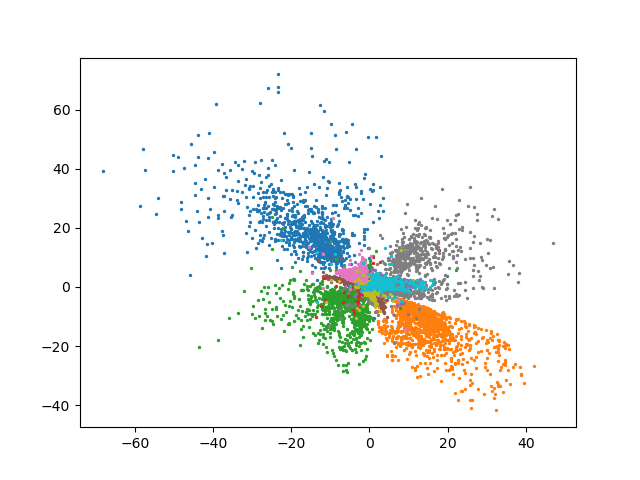
\includegraphics[width=12cm]{images/ae_2dims_latent_variables.png}
    \caption{Autoencoders' latent variables}
    \label{fig:ae_2dims_latent_variables}
\end{figure}

\subsection{Activations}

\subsection{Filters/Kernels}
Visualize the convolutional kernels.
\subsubsection{AlexNet}
\begin{itemize}
    \item \textbf{conv2d/0}, $[64, 3, 11, 11]$
    \item \textbf{conv2d/1}, $[192, 64, 5, 5]$
    \item \textbf{conv2d/2}, $[384, 192, 3, 3]$
    \item \textbf{conv2d/3}, $[256, 384, 3, 3]$
    \item \textbf{conv2d/4}, $[256, 256, 3, 3]$
\end{itemize}

\begin{figure}[H]
    \centering
    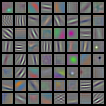
\includegraphics[width=8cm]{images/alexnet_0_kernels.png}
    \caption{conv2d/0@[64, 3, 11, 11] (colorful)}
    \label{fig:alexnet_0_kernels}
\end{figure}

\begin{figure}[H]
    \centering
    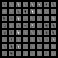
\includegraphics[width=8cm]{images/alexnet_1_1_kernels.png}
    \caption{conv2d/1: first kernel@[64, 5, 5]}
    \label{fig:alexnet_0_kernels}
\end{figure}

\subsection{Gradient}
\subsection{Class specific image generation}